% Sumber: reports/audit_summary_metrics.csv, reports/audit_per_skin_tone_accuracy.csv,
% reports/preprocessing_experiment_summary.csv (melalui docs/EXPERIMENT.md EXP-006),
% reports/arcface_evaluation/{comparison_metrics,statistical_tests,skin_tone_analysis}.csv,
% reports/arcface_error_analysis/neutral_error_analysis.csv, docs/EXPERIMENT.md,
% docs/EXP-007_ARCFACE_EVALUATION.md, research-audit/DATA_DISCREPANCIES.md (D-8).
\chapter{Hasil dan Pembahasan}
\label{chap:results}

Bab ini menjawab RQ1, RQ2, dan RQ3 secara berurutan. Setiap bagian tetap berada dalam populasinya sendiri: 227 potongan, tujuh-kelas, untuk RQ1 dan RQ2; subset 135 potongan, lima-kelas, untuk RQ3. Tidak satu pun menggabungkan angka dari satu populasi dengan angka dari populasi lain tanpa menyatakannya secara eksplisit.

\section{RQ1: Karakteristik Kesalahan Garis Dasar HSEmotion pada Sampel 227 Potongan}
\label{sec:rq1-results}

Keluaran HSEmotion (model terlatih, dipakai apa adanya) pada 227 potongan tanpa modifikasi mencapai akurasi keseluruhan 22,47\% terhadap kebenaran lapangan satu-anotator, dengan 17,62\% dari seluruh 227 prediksi berupa panggilan ``Marah'' yang salah (Marah diprediksi padahal label aslinya bukan itu). Memecah tingkat salah-Marah ini berdasarkan label asli menunjukkan di mana ia terkonsentrasi: 18 dari 76 potongan berlabel-asli Netral (23,7\%) diprediksi Marah, yang merupakan pola kesalahan tunggal terbesar yang bisa diidentifikasi pada sampel ini, lebih besar, dalam hitungan mutlak, dibanding pasangan kebingungan (\textit{confusion}) lain mana pun.

Dua kelompok proksi warna kulit yang dikarakterisasi pada sampel ini menunjukkan akurasi yang mencolok bedanya: 44,0\% untuk potongan Gelap berbanding 14,3\% untuk potongan Gelap-Sedang, selisih 29,7 poin persentase (dihitung sebagai selisih maksimum-dikurangi-minimum sederhana antara dua kelompok ini, bukan ukuran efek yang dinormalisasi atau metrik keadilan tingkat-populasi). Uji eksak Fisher pada data yang sama menghasilkan rasio odds 5,88 ($p = 0,0027$), yang mendukung bahwa kelompok ini dan hasil klasifikasi berasosiasi secara statistik pada sampel ini. Hasil ini tidak mendukung pembacaan sebab-akibat. Kedua kelompok ini adalah statistik kecerahan yang dihitung per potongan, bukan ukuran demografis yang tervalidasi (Bab~\ref{chap:methodology} \S\ref{sec:dataset-overview}), dan tidak ada apa pun dalam rancangan sampel ini (satu film sumber, satu kamera, satu tata pencahayaan, tanpa pengacakan dalam bentuk apa pun) yang memisahkan variabel proksi ini dari faktor-faktor yang berkorelasi, seperti adegan mana yang kebetulan menjadi sumber potongan tiap kelompok. Asosiasi sekuat ini layak dilaporkan secara presisi; asosiasi ini, dengan sendirinya, bukanlah penjelasan.

Ada satu catatan yang lebih pantas ditulis di sini daripada di catatan kaki. \textit{Notebook} ablasi-CLAHE milik proyek ini sendiri (EXP-006) memuat perhitungan per-kelompok-warna-kulit kedua yang dihitung secara independen, dan angka ``sebelum''-nya, yaitu pada potongan tanpa modifikasi, untuk dua kelompok yang sama adalah 27,7\% (Gelap) dan 10,8\% (Gelap-Sedang), bukan 44,0\% dan 14,3\%, meskipun kedua \textit{notebook} melaporkan akurasi keseluruhan yang identik, 22,47\%, untuk kondisi yang seharusnya sama. Perbedaan ini dicatat lengkap pada \texttt{research-audit/DATA\_DISCREPANCIES.md} (butir D-8) dan belum terselesaikan pada revisi ini. Logika pengelompokan per-baris pada kedua \textit{notebook} tersebut belum diperiksa langsung, karena berkas CSV mentah dari keduanya tidak tersedia untuk diturunkan ulang dalam repositori ini. Tesis ini melaporkan angka EXP-005 di atas sebagai nilai acuan, karena EXP-005 adalah audit warna kulit yang memang dirancang khusus untuk itu, sedangkan perhitungan pada EXP-006 adalah keluaran sampingan dari ablasi yang tujuannya berbeda; tesis ini tidak mengklaim bahwa kedua \textit{notebook} ini saling mengonfirmasi, karena pada perhitungan spesifik ini keduanya jelas-jelas tidak sama.

Apa yang terbukti dan apa yang tidak terbukti, dinyatakan secara gamblang: terbukti bahwa model ini, pada sampel ini, berkinerja jauh di bawah yang biasa dilaporkan pada benchmark-nya sendiri, dengan satu kesalahan yang spesifik dan cukup besar, terkonsentrasi pada satu kelas ekspresi dan satu arah kebingungan. Tidak terbukti mengapa, baik untuk akurasi agregat yang rendah, maupun untuk selisih proksi warna kulit, dan tidak terbukti apa pun tentang perilaku model ini terhadap wajah masyarakat Papua sebagai sebuah populasi, karena 227 potongan dari satu film bukanlah sampel yang dirancang untuk mendukung generalisasi semacam itu.

\section{RQ2: Pengaruh Konfigurasi CLAHE yang Diuji}
\label{sec:rq2-results}

Menerapkan varian CLAHE adaptif yang dijelaskan pada Bab~\ref{chap:methodology} \S\ref{sec:clahe-config} pada 227 potongan yang sama, lalu menjalankan ulang model HSEmotion beku yang sama, mengubah akurasi keseluruhan dari 22,47\% menjadi 19,82\% dan tingkat salah-Marah dari 17,62\% menjadi 18,06\%. Kedua angka ini bergerak ke arah yang berlawanan dengan dugaan hipotesis eksperimen itu sendiri: judul \textit{notebook} sumbernya sendiri menyatakan bahwa uji ini dimaksudkan untuk melihat apakah CLAHE akan mengurangi prediksi salah-Marah dan memperbaiki kesetaraan antar-proksi warna kulit, dan pada jalan uji ini CLAHE tidak melakukan keduanya.

\begin{figure}[htbp]
\centering
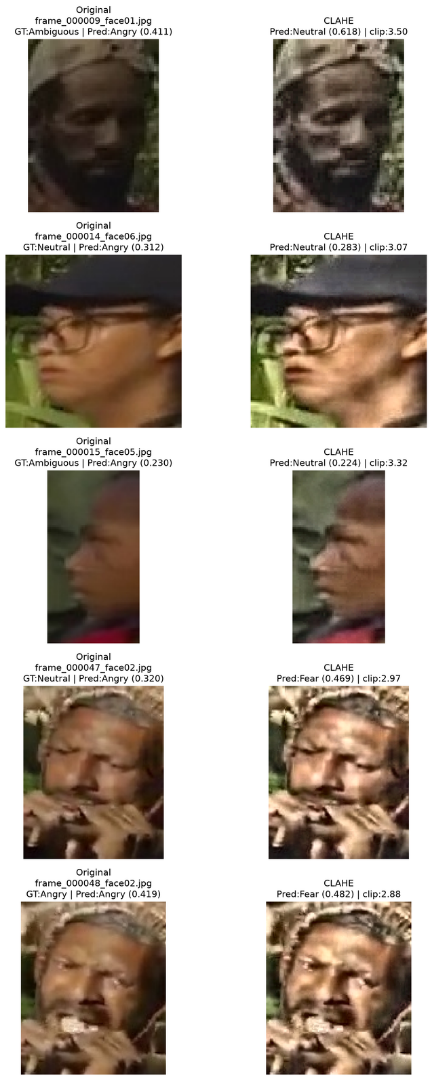
\includegraphics[width=0.35\textwidth]{figures/perbandingan-clahe-sebelum-sesudah}
\caption[Contoh kualitatif potongan wajah sebelum dan sesudah CLAHE]{Contoh kualitatif perbandingan potongan wajah asli (kiri) dan hasil olahan CLAHE (kanan), dengan label kebenaran lapangan (GT), prediksi HSEmotion, dan nilai batas klip (\textit{clip limit}) adaptif yang dipakai untuk tiap potongan. Batas klip terlihat bervariasi antar-potongan (2,88 hingga 3,50), sesuai mekanisme yang dijelaskan pada \S\ref{sec:clahe-config}: batas klip menyesuaikan estimasi kecerahan tiap potongan secara individual, bukan nilai tetap untuk seluruh sampel. Gambar ini untuk ilustrasi mekanisme saja; angka akurasi agregat 22,47\%$\to$19,82\% di atas dihitung atas seluruh 227 potongan, bukan hanya lima contoh yang ditampilkan di sini.}
\label{fig:clahe-contoh}
\end{figure}

Gambar~\ref{fig:clahe-contoh} menunjukkan efek visual CLAHE pada beberapa contoh potongan: kontras memang berubah, dan pada beberapa contoh prediksi model ikut berubah (misalnya dari ``Angry'' menjadi ``Neutral'' atau ``Fear''), tetapi perubahan tersebut tidak konsisten ke satu arah, sejalan dengan angka agregat di atas yang menunjukkan hasil bersihnya justru sedikit memburuk, bukan membaik.

Ini adalah satu kali eksekusi tanpa pengulangan, dan tanpa selang kepercayaan atau uji signifikansi yang dihitung untuk kedua selisih tersebut (Bab~\ref{chap:methodology} \S\ref{sec:clahe-config}). Penurunan akurasi 2,65 poin persentase dan kenaikan salah-Marah 0,44 poin, yang teramati satu kali saja, tidak membuktikan bahwa konfigurasi CLAHE tertentu ini merugikan dengan keyakinan statistik apa pun, apalagi bahwa CLAHE sebagai teknik praproses pada umumnya merugikan. Rentang batas klip yang berbeda, pemetaan kecerahan yang berbeda, atau sekadar variasi acak dari pengulangan sampel, semuanya bisa saja, pada prinsipnya, menggeser hasil ini. Yang didukung oleh pengamatan ini, pada lingkup yang benar-benar diukur, lebih sempit dan tetap layak dinyatakan secara langsung: untuk konfigurasi CLAHE adaptif ini, model ini, dan sampel ini, langkah praproses tersebut tidak memberikan perbaikan yang menjadi tujuan pengujiannya, dan seorang peneliti yang harus memilih antara memakai konfigurasi ini atau tidak, tidak akan menemukan bukti di sini yang membenarkan pemakaiannya.

\section{RQ3: HSEmotion Berbanding Regresi Logistik Berbasis ArcFace pada Subset 135 Potongan}
\label{sec:rq3-results}

\textbf{Perbandingan ini dijalankan sebelum versi apa pun dari pertanyaan penelitian tesis ini ditulis.} Hasil ini dilaporkan di sini sebagai analisis retrospektif atas bukti yang sudah ada sebelumnya, menjawab RQ3 belakangan, bukan sebagai uji konfirmatif yang memang dirancang di muka untuk menghasilkan RQ3 (Bab~\ref{chap:introduction} \S\ref{sec:rq}). Perbedaan ini memengaruhi seberapa besar bobot yang semestinya diberikan pada hasil di bawah ini: hasil yang diperoleh dengan cara ini tetaplah bukti yang sah, tetapi bobot konfirmatifnya lebih kecil dibanding perbandingan yang dirancang di muka khusus untuk menjawab pertanyaan tersebut.

\begin{table}[h]
\centering
\caption[Perbandingan HSEmotion dan ArcFace+Regresi Logistik]{HSEmotion berbanding ArcFace+Regresi Logistik, subset 135 potongan, lima kelas. Sumber: berkas hasil evaluasi ArcFace (metrik perbandingan dan uji statistik) pada proyek ini.}
\label{tab:rq3-comparison}
\begin{tabular}{lrr}
\toprule
Metrik & HSEmotion & ArcFace + LR \\
\midrule
Akurasi & 36,30\% & 40,74\% \\
Presisi makro & 0,590 & 0,280 \\
\textit{Recall} makro & 0,206 & 0,293 \\
F1 makro & 0,249 & 0,272 \\
SK 95\% \textit{bootstrap} (akurasi, sadar-kelompok) & [0,269, 0,467] & [0,338, 0,481] \\
\bottomrule
\end{tabular}
\end{table}

Akurasi titik ArcFace+LR (40,74\%) secara angka lebih tinggi dari HSEmotion (36,30\%) pada subset ini, tetapi uji McNemar pada 46 prediksi yang tidak sepakat (20 berpihak pada ArcFace+LR, 26 berpihak pada HSEmotion) menghasilkan $p = 0,4614$: tidak ada perbedaan yang terdeteksi pada tingkat signifikansi yang lazim. Inilah seluruh klaim dari hasil ini: uji McNemar yang tidak signifikan pada ukuran sampel ini berarti perbedaannya tidak terdeteksi, bukan berarti kedua klasifier setara. Dengan hanya 46 pasangan yang tidak sepakat sebagai bahan uji, perbedaan nyata yang ukurannya sedang-sedang saja bisa dengan mudah luput terdeteksi di sini; tesis ini tidak membaca hasil nihil ini sebagai temuan bahwa kedua pendekatan berkinerja sama.

Angka presisi/\textit{recall}/F1 makro tidak menunjukkan satu klasifier yang unggul di segala aspek: presisi makro HSEmotion lebih tinggi, sementara \textit{recall} dan F1 makro ArcFace+LR lebih tinggi. Ini sejalan dengan dugaan bahwa kedua klasifier membuat jenis kesalahan yang berbeda, bukan satu klasifier yang sekadar membuat lebih sedikit kesalahan dibanding yang lain. Perbedaan ini terlihat langsung pada bagaimana masing-masing model menangani kelas Netral, kelas terbesar dalam subset ini (76 dari 135 potongan): HSEmotion salah mengklasifikasi 34 dari 76 potongan Netral, dan kesalahan tersebut terkonsentrasi kuat ke satu arah, 18 di antaranya berlabel Marah. ArcFace+LR salah mengklasifikasi lebih banyak potongan Netral (43 dari 76) tetapi menyebarkannya ke empat kelas lain (Senang 15, Sedih 14, Takut 8, Terkejut 6) tanpa satu target kebingungan yang dominan. Klasifier yang membuat lebih banyak kesalahan total tetapi menghindari satu pola kegagalan yang timpang tidak serta-merta lebih buruk untuk semua keperluan, dan tesis ini tidak mengurutkan kedua pendekatan hanya berdasarkan akurasi semata.

Pada perhitungan proksi warna kulit dalam subset 135 potongan yang sama ini, kedua klasifier mencapai akurasi 45,65\% pada kelompok Gelap ($n=46$); pada kelompok Gelap-Sedang ($n=32$), ArcFace+LR mencapai 31,25\% berbanding 12,50\% milik HSEmotion, selisih antar-kelompok proksi yang lebih kecil untuk ArcFace+LR (14,4 poin) dibanding HSEmotion (33,2 poin) pada subset ini. Ini adalah satu pengamatan tunggal yang belum direplikasi pada satu kelompok berisi 32 potongan, bukan perbaikan keadilan yang sudah terbukti, dan tesis ini tidak memakainya sebagai bukti perbaikan keadilan. Hasil ini dilaporkan karena memang bagian dari apa yang ditunjukkan data, dengan bobot yang persis sebesar itu saja.

\section{Papuan V2: Status, Bukan Hasil}
\label{sec:rq-papuanv2-status}

Belum ada temuan kuantitatif dari jalur Papuan V2 yang layak masuk bab hasil, karena memang belum ada. Ekstraksi berskala uji-coba 645 potongan sudah selesai; uji coba anotasi label emosi belum (antrean anotator tumpang-tindih menunjukkan nol dari 75 tugas selesai pada status terakhir yang tercatat, dan klaim penyelesaian anotator utama belum diverifikasi ulang secara independen, \texttt{research-audit/DATA\_DISCREPANCIES.md} D-1); uji coba titik-fitur CVAT 24-gambar baru berisi usulan otomatis dan belum diperiksa manusia. Tidak satu pun dari RQ1 sampai RQ3 memakai jalur ini sebagai bukti, dan bagian ini ada semata agar pembaca tidak perlu menyimpulkan sendiri ketiadaannya dari keheningan. % TODO: isi dengan tabel hasil, berstruktur seperti Tabel~\ref{tab:rq3-comparison}, hanya setelah uji coba CVAT diperiksa dan dataset yang dihasilkan dievaluasi pada partisi uji yang disisihkan, bukan sebelum itu.

\section{Sintesis}

RQ1 dan RQ2 menjelaskan populasi 227 potongan yang sama di bawah dua kondisi praproses; RQ3 menjelaskan subset 135 potongan dari populasi yang sama di bawah dua klasifier. Jika dibaca bersama: akurasi HSEmotion pada sampel ini rendah dibanding kinerja yang biasa dilaporkan pada benchmark-nya, disertai selisih akurasi proksi warna kulit yang spesifik, besar, dan berasosiasi secara statistik (tidak terbukti sebab-akibat), serta pola kesalahan Netral-menjadi-Marah yang dominan dan tetap sama baik diukur pada 227 maupun 135 potongan; satu konfigurasi CLAHE yang diuji tidak membantu, dalam satu kali jalan uji yang tidak terkontrol; dan perbandingan retrospektif terhadap alternatif berbasis ArcFace tidak menemukan perbedaan akurasi keseluruhan yang signifikan secara statistik, disertai sebaran kesalahan yang secara kualitatif berbeda dan tidak setimpang untuk klasifier alternatif tersebut. Tidak satu pun dari ini berlaku umum melampaui satu film sumber sampel ini, dan tidak satu pun dari ini menjadi bukti tentang jalur Papuan V2, yang tetap merupakan pekerjaan terpisah dan belum selesai.
